\TNchapter[Capability is half the picture. The other half is whether the agent answers in time, costs less than the work it replaces, and survives the day after launch. This chapter covers the operational benchmarks your CFO will care about: latency at the tail, throughput under load, and outcome-normalized cost as a worked example. It also makes the case that the latency number Maya's team is going to quote her (the median) is not the one her users are going to feel. The one they feel is the 99th percentile, and it is usually the one no one measured.]{Speed, cost, and scale}
\label{ch:30-benchmarking-11-speed-cost}

\starttwocol

\section{Latency is the number that doesn't average}

A vendor demo will show an agent that responds in 1.2 seconds. Your team will time it again and see 1.4 seconds. The deck will round to ``about a second'' and everyone will move on. By the time the agent ships and an angry customer is on the phone, the actual response they waited through was 22 seconds, and no one knows why because no one was measuring the right number.

The number the vendor showed you was the median. The number the angry customer experienced was the 99th percentile. They are not the same number, and the gap between them is usually larger than anyone expects.

\begin{TNdefinition}{Latency p50, p95, p99} the response-time percentiles. p50 is the median; half of requests are faster, half are slower. p95 is the value below which 95\% of requests fall; the other 5\% are slower than this. p99 is the same for 99\%. The first is what your team will quote; the last is what your users will feel. \end{TNdefinition}

\begin{TNdefinition}{TTFT (time to first token)} for streaming agents, the time from request to the first character of response. Distinct from total latency. A 6-second response that starts streaming at 400ms feels fast; a 2-second response that streams nothing for 1.8 seconds and then dumps the whole answer feels slow. Optimize TTFT separately. \end{TNdefinition}

The tail latency --- the slow end of the distribution --- is the part your users actually notice. Most users will not register the difference between a 600 ms response and an 800 ms one. They will absolutely register a 22-second response that arrives after they've already started typing again. p95 and p99 are not engineering preferences. They are product decisions.

\begin{figure*}[tb]
\centering
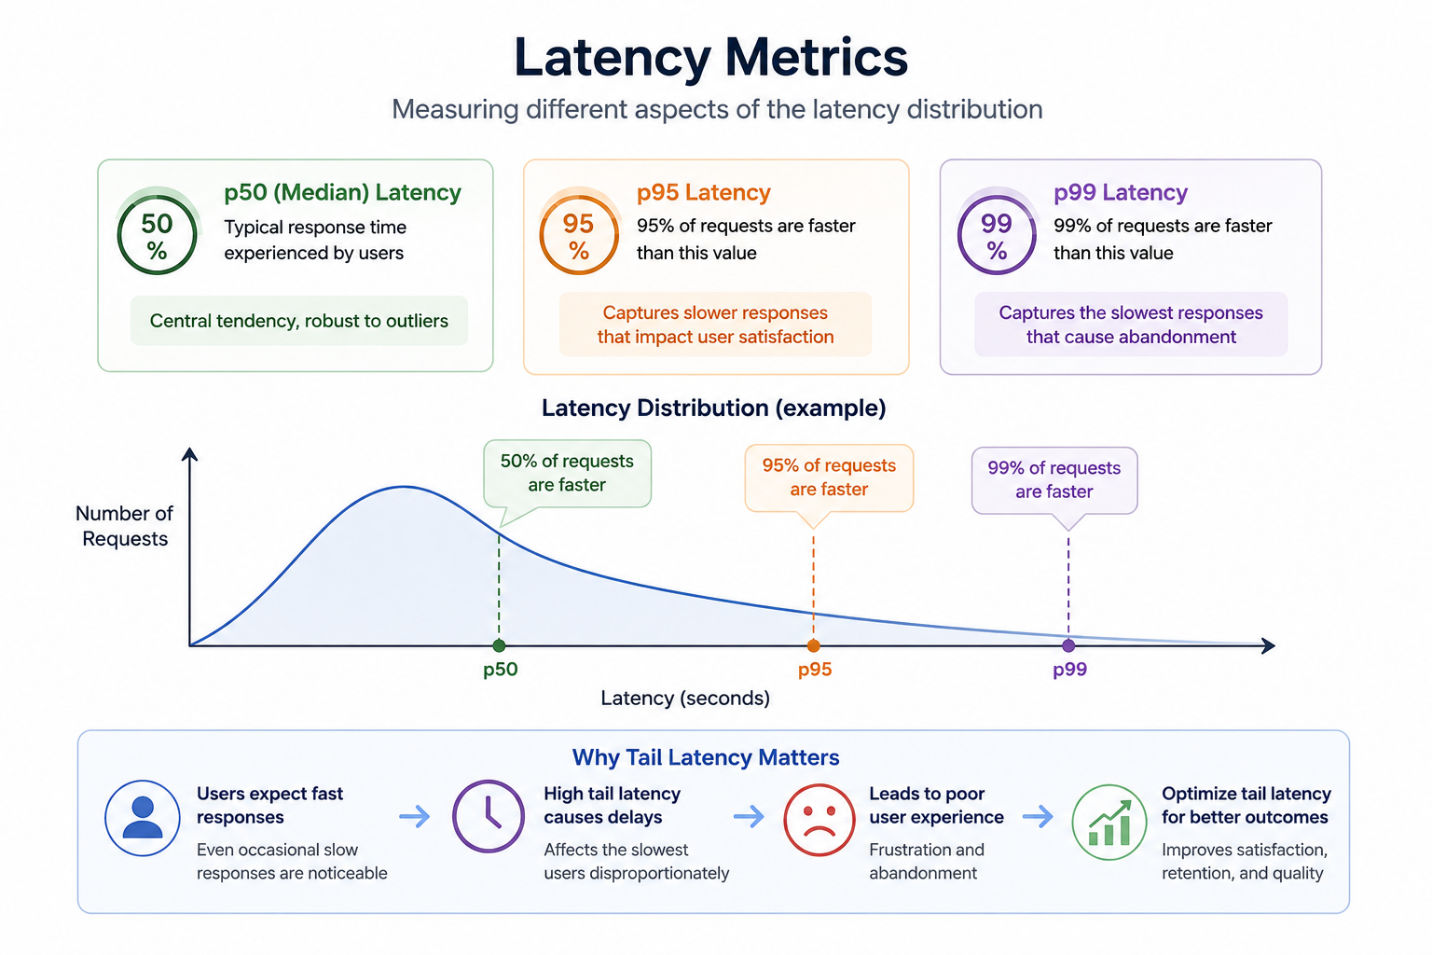
\includegraphics[width=0.9\textwidth]{figures/benchmarking/latency-p50-p95-p99.png}
\caption{Latency metrics: p50/p95/p99 distribution and why tail latency matters for user experience.}
\end{figure*}

A useful rule for Maya's team: measure p50, p95, and p99. Quote p99 to the product team. If the gap between p50 and p99 is wider than 5x, you have a tail problem, and it will get worse under load.

\section{Throughput, and why ``low latency at low load'' is a lie}

The other operational number is throughput: how many agent requests the system can serve per second without slowing down. Throughput and latency are related and frequently confused.

A pilot with five users in a conference room will look fast. A production rollout to two thousand users will not. Between those two states, every queueing delay, every shared resource bottleneck, every retry storm in the agent's tool calls becomes visible. The pilot number tells you what the agent can do when nothing is in its way. The production number tells you what the agent does when everything is.

For Maya: ask your team for two numbers, not one. The first is latency at the pilot load (say, ten concurrent users). The second is latency at the projected production load (say, two thousand). If the team only has the first, you don't have a deployment plan; you have a hope.

\section{Token economics --- why generation speed is a deployment metric}

The agent's economics are mostly about tokens. Every prompt sent to the model is paid in input tokens; every response is paid in output tokens; multiplied by the volume your agent processes per day, the bill is the bill.

Two technical realities shape what your team can do about that bill. The first is the \textit{prefill / decode split}: an agent's response time is dominated by two phases --- prefill (the model reading the prompt) and decode (the model generating the response, one token at a time). Decode is sequential and usually slower per token. Long prompts cost mostly prefill; long responses cost mostly decode. Optimizing one without the other is a common mistake.

The second is that the inference-cost frontier has moved. In 2024--25, three families of inference-side techniques cut token-generation cost by 2x--4x in production deployments. These are not your team's choices to make most of the time --- the model vendor makes them --- but they should show up in any vendor comparison your team does on cost.

\begin{TNinpractice}{Inference-side cost levers (2024--25)} \textit{Speculative decoding} uses a smaller model to draft tokens that a larger model verifies in batches. \textit{Paged attention} gives the KV cache a more efficient memory layout. Aggressive \textit{KV cache reuse} shares cached attention across requests. Each is a vendor-side optimization; together they account for most of the per-token price drop your team has seen on its 2025 bill. \end{TNinpractice}

\begin{TNwarning} Be skeptical of vendor cost projections that assume current per-token pricing will hold for the life of the contract. The price has fallen by an order of magnitude over the last twenty-four months, and is likely to keep falling. The agent that wins on cost today may lose on switching cost tomorrow if your team has overfit to one vendor's pricing model. \end{TNwarning}

\section{Cost-per-outcome, not cost-per-call}

The single most consequential reframe in this Part is the one \autoref{ch:30-benchmarking-09-strategy} introduced: the right cost metric is cost per \textit{resolved business outcome}, not cost per token or per call. Here is the formal version.

\begin{TNdefinition}{Outcome-normalized cost} the total cost (model tokens, tool calls, infrastructure, human intervention) divided by the number of successful business outcomes (resolved tickets, closed cases, correct decisions). The denominator is the work done; the numerator is everything it took to do it. A \$0.30-per-call agent that resolves 95\% of tickets first time is cheaper than a \$0.05-per-call agent that needs five tries. \end{TNdefinition}

\begin{figure*}[tb]
\centering
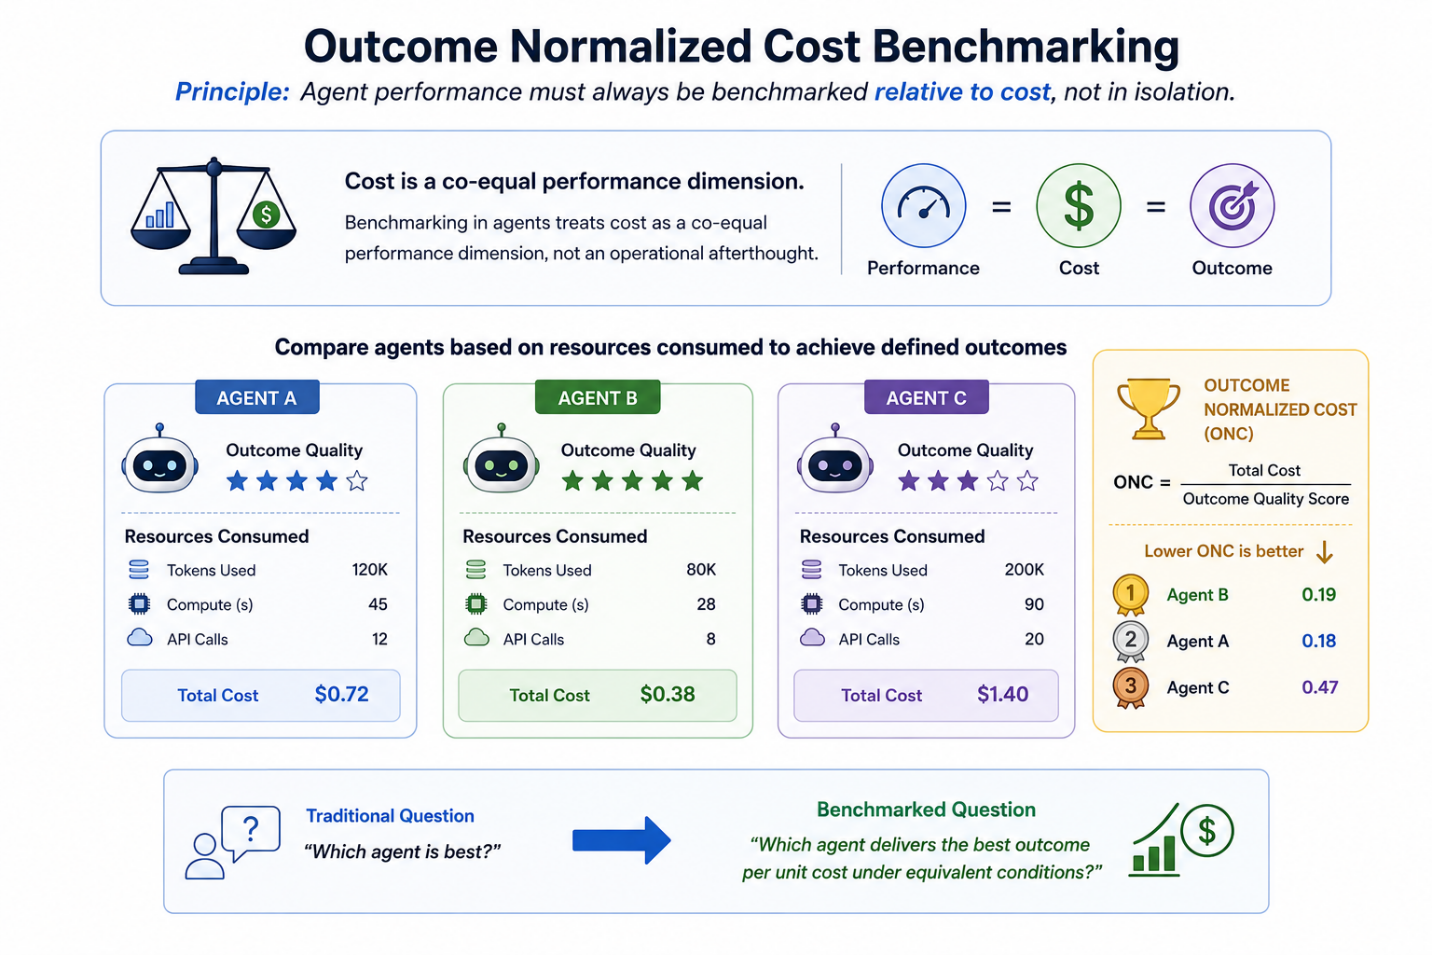
\includegraphics[width=0.9\textwidth]{figures/benchmarking/outcome-normalized-cost.png}
\caption{Outcome-normalized cost benchmarking: comparing agents on resources consumed per defined outcome.}
\end{figure*}

The worked example is the cleanest way to see why this matters. Consider three configurations of the same agent, benchmarked on the same workload of customer-service tickets \textit{(figures illustrative)}:

\begin{table*}[tb]
\centering
\small
\begin{tabular}{@{}lcccc@{}}
\toprule
\textbf{Agent variant} & \textbf{Task success rate} & \textbf{Avg cost per task} & \textbf{Avg latency} & \textbf{Cost per successful outcome} \\
\midrule
Agent v1 & 92\% & \$0.42 & 3.1 s & \$0.46 \\
Agent v2 & 95\% & \$0.68 & 2.4 s & \$0.72 \\
Agent v2 (low-cost mode) & 90\% & \$0.29 & 4.9 s & \$0.32 \\
\bottomrule
\end{tabular}
\caption{Three configurations of the same agent on the same workload of customer-service tickets (illustrative figures).}
\end{table*}

Read this table once. The first instinct --- ``Agent v2 has the highest accuracy, ship it'' --- is wrong for almost every workload that matters. Agent v2 (low-cost mode) costs less than half as much per resolved outcome as Agent v2 and a third less than Agent v1. For a workload of a million tickets a year, the gap between v2 and v2 (low-cost) is \$400,000 per year, paid for five percentage points of accuracy. Whether that is worth paying depends on what those five points are doing.

The decision is now negotiable. If the missed 10\% in v2 (low-cost) are easy escalations that go cleanly to a human agent, the low-cost variant wins. If the missed 10\% are catastrophic errors that mishandle a refund, v2 wins on cost too once you count the cleanup. Outcome-normalized cost forces this conversation to happen before the contract is signed, not after.

\begin{TNinpractice}{Meridian Logistics} \textit{A third-party logistics provider (3PL) whose quote-generation agent answered in 2.2 seconds at p50 in pilot.} The team shipped it. Two months later, customers in Atlanta were reporting waits of 28 seconds --- the p99 --- because a traffic spike from a new B2B integration was hitting the tail. The fix was not faster inference. The fix was a routing tier: cheap, deterministic responses for the 70\% of requests that matched a known pattern, agent inference for the remaining 30\%. Cost per resolved quote dropped 40\%; p99 dropped from 28 seconds to 4 seconds. The agent didn't get smarter. The system got smarter about when to use it. \end{TNinpractice}

\section{Load and stress testing --- what changes between 100 users and 100{,}000}

The last operational discipline is load testing. The point of load testing is not to find the breaking point. The point is to find the \textit{behavior change} point --- the load at which the agent's pattern of failures changes shape.

A well-behaved agent serves a thousand requests with similar latency to one. A less well-behaved agent serves a thousand with similar latency to one, then suddenly serves the next hundred with latency ten times higher, because some shared resource (a vector database, a tool gateway, a model-provider rate limit) has tipped over. Load testing finds these tipping points before your customers do.

\begin{TNdefinition}{Load testing vs. stress testing} load testing measures behavior at expected and elevated traffic levels, looking for degradation curves. Stress testing deliberately overloads the system to find failure modes and recovery behavior. Load testing answers ``will it hold?''; stress testing answers ``how does it break?'' You need both. \end{TNdefinition}

The third concept worth knowing is \textit{denial-of-wallet}: the cost-side cousin of denial-of-service. Where a denial-of-service attack tries to take an agent offline, a denial-of-wallet attack tries to drive up the agent's token spend until the bill exceeds what the business can sustain. The defenses are different from denial-of-service defenses --- per-user rate limits on token spend, anomaly detection on cost per session, hard caps on the agent's tool-call budget per turn. Chapter 6 names the attack; the operational discipline lives here.

\begin{TNwarning} A ``low latency at low load'' benchmark tells you nothing about production behavior. If your team's only latency number was taken in a pilot, demand a second number under projected production load before signing off on a deployment. \end{TNwarning}

\section{What the CFO will ask, in advance}

When the agent goes to budget review, three questions will land in your CFO's inbox before they land in yours. Have the answers ready.

The first: \textit{what does this agent cost per resolved outcome, and how does that compare to the cost of doing the work without it?} Anything that is not in that form --- cost per token, cost per call, cost per ``interaction'' --- is a question your CFO will see through. Outcome-normalized cost is the only number that survives finance review.

The second: \textit{what does the cost look like at 10x volume?} The token-cost component scales linearly. The model-provider rate limits, the infrastructure, the human-review overflow do not. The 10x answer is usually not 10x the cost; it is somewhere between 6x (if the agent scales cleanly) and 25x (if it doesn't). Your team should know which.

The third: \textit{what does the cost look like in six months, if the model is upgraded twice?} The vendor pricing today is unlikely to be the vendor pricing in six months. The contract terms matter as much as the per-token cost.

\section{The other meter: people}

Token cost is the meter every team learns to read. It is also the meter that under-reports the bill by roughly an order of magnitude. The agent's true unit cost is dominated by the humans you have to keep around to make sure the agent does not embarrass you on a Sunday night.

The Google SRE book is the cleanest scaffold here, and the numbers transfer \citep{google-sre-book}. A service that runs 24/7 needs at least eight engineers on a single-site rotation to be on-call sustainably, or six per site for a two-site follow-the-sun. Below that, you are not running an on-call; you are running a burnout pipeline. Of an SRE's time, the workbook is explicit: at least 50\% goes to engineering, no more than 25\% to on-call, and the remainder to other operational work. A shift that absorbs more than two incidents is, by Google's own math, over capacity --- each incident is budgeted at roughly six hours of root cause, remediation, and postmortem.

Layer the agent-specific overhead on top. Industry TCO writeups converge on a rule of thumb of \textbf{0.25 to 0.5 FTE of an AI engineer per non-trivial production agent} for prompt upkeep, eval refresh, and model-version churn --- the work \autoref{ch:10-alignment-04-oversight} called \textit{behaviour drift}. At a fully loaded \$300K, that is \$75K to \$150K per agent per year, before SRE, before the reviewer pool from \autoref{ch:10-alignment-04-oversight}, before vendor observability, before retraining inference cost.

A working rule for a medium-tier agent, before tuning to your numbers: \textbf{0.5 SRE plus 0.25 AI engineer plus the reviewer pool that the escalation rate implies, with a 30\% on-cost for vacation, training, and bench}. A high-tier agent doubles the SRE share and adds a named on-call ML engineer. McKinsey's \textit{State of AI 2025} reports that high-performing companies allocate more than 20\% of their digital budget to AI, against 7\% for the rest \citep{mckinsey-state-of-ai-2025}; the gap is mostly people, not tokens.

The CFO's question is not \textit{what does the agent cost per call}. It is \textit{what does the agent cost per call divided by the team it takes to keep it running}. Get both numbers before the budget conversation.

\TNrule

\stoptwocol

\begin{TNkeytakeaways}
\item The latency you should quote is p99, not p50. The gap between them is the one your users feel.
\item Throughput and latency together --- at production load, not pilot load --- are the only honest performance signal.
\item Cost per resolved outcome, not cost per call, is the number that decides whether the agent pays for itself.
\item Token economics shift faster than agent contracts. Plan for prices to fall and the cost frontier to move underneath your deployment.
\item Load testing finds the curve; stress testing finds the cliff. You need both.
\end{TNkeytakeaways}

\begin{TNchecklist}
\item Require p99 (not just p50) for every latency claim in every vendor comparison.
\item Run a load test at projected production volume before sign-off; refuse to ship without one.
\item Make outcome-normalized cost --- dollars per resolved business outcome --- the headline cost metric in every agent deck.
\item For any conversational agent, characterize TTFT separately from total latency; the first is the perception, the second is the bill.
\item Set a per-session and per-day token-spend cap as a denial-of-wallet defense.
\item Re-run your cost benchmark on a quarterly cadence; vendor pricing and model efficiency both move.
\item Demand both the ``happy path'' cost and the ``10x volume'' cost in any vendor proposal.
\end{TNchecklist}



